\chapter{Sistema Desenvolvido}
\label{chap:sistema-desenvolvido}

texto texto texto

\section{Aquisição de Dados}
\label{sec:aquisicao-dados}

    oi
    
    \subsection{Métodos de Aquisição}
    \label{sec:metodos-aquisicao}
        oi
        
        \subsubsection{HTTP}
        \label{sec:aquisicao-http}
        oi
        
        \begin{figure}[!h]
		\Caption{\label{fig:figura-http-geral} Diagrama das etapas do servidor para manipulação de dados.}
		%\centering
		\UFCfig{}{
			\fbox{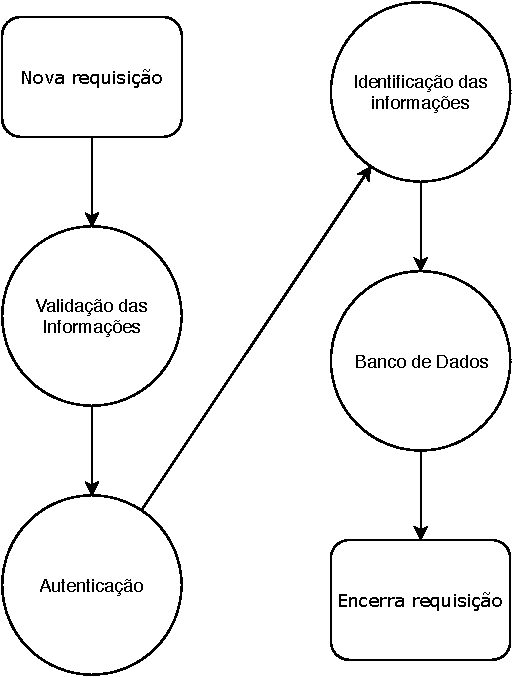
\includegraphics[width=8cm]{figuras/http-geral.pdf}}
		}{
			\Fonte{O autor}
		}	
    	\end{figure}
    	
    	\begin{figure}[!h]
		\Caption{\label{fig:figura-http-validacao} Diagrama de validação das informações recebidas.}
		%\centering
		\UFCfig{}{
			\fbox{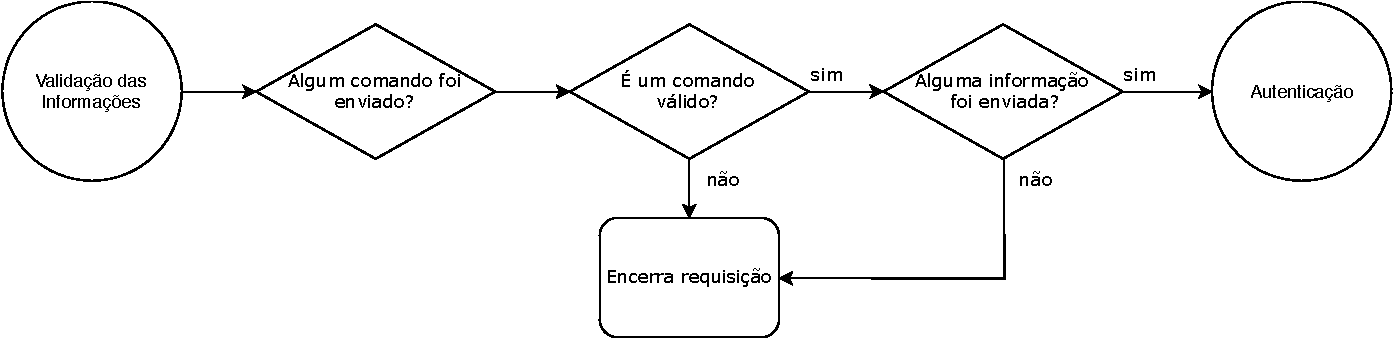
\includegraphics[width=15cm]{figuras/http-validacao.pdf}}
		}{
			\Fonte{O autor}
		}	
    	\end{figure}
    	
    	\begin{figure}[!h]
		\Caption{\label{fig:figura-http-autenticacao} Diagrama de autenticação do usuário.}
		%\centering
		\UFCfig{}{
			\fbox{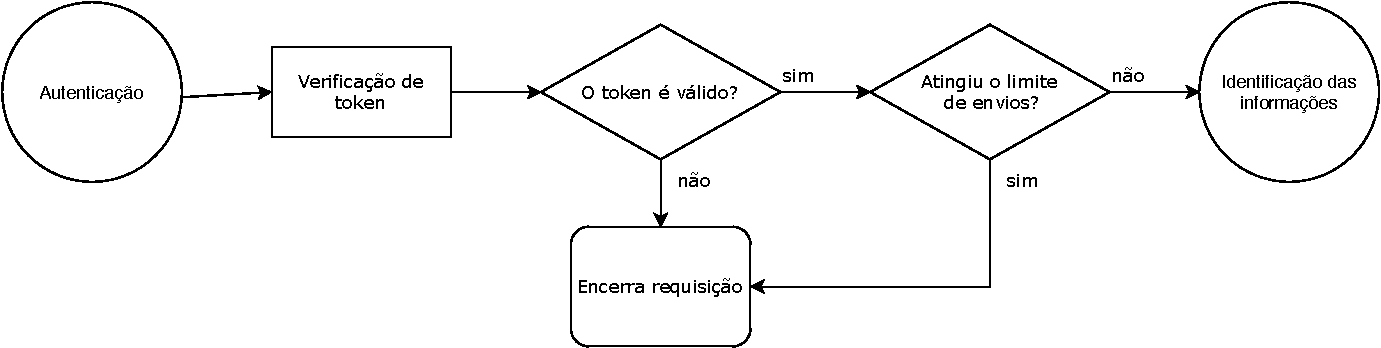
\includegraphics[width=15cm]{figuras/http-autenticacao.pdf}}
		}{
			\Fonte{O autor}
		}	
    	\end{figure}
    	
    	\begin{figure}[!h]
		\Caption{\label{fig:figura-http-identificacao} Diagrama sobre a identificação do tipo das informações.}
		%\centering
		\UFCfig{}{
			\fbox{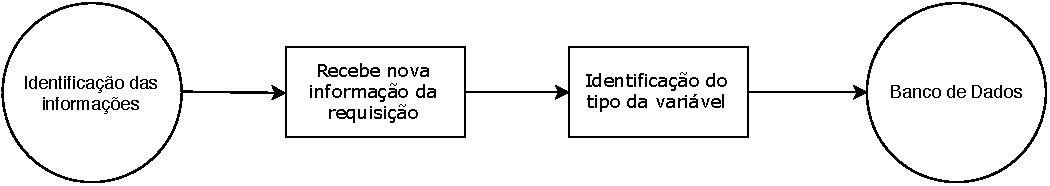
\includegraphics[width=15cm]{figuras/http-identificacao.pdf}}
		}{
			\Fonte{O autor}
		}	
    	\end{figure}
    	
    	\begin{figure}[!h]
		\Caption{\label{fig:figura-http-banco} Banco de Dados.}
		%\centering
		\UFCfig{}{
			\fbox{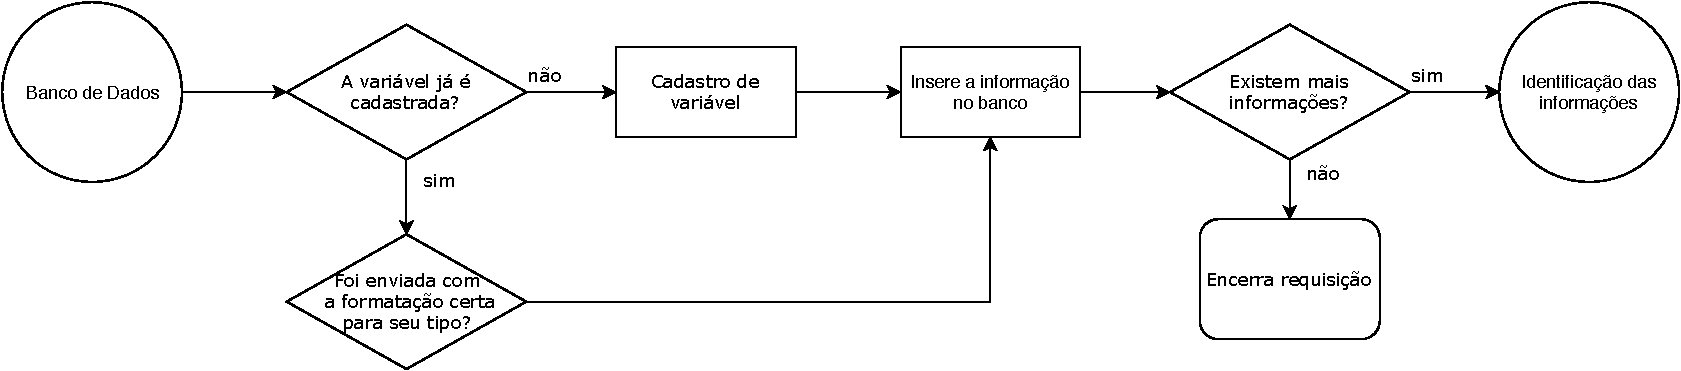
\includegraphics[width=15cm]{figuras/http-banco.pdf}}
		}{
			\Fonte{O autor}
		}	
    	\end{figure}
        
        \subsubsection{MQTT}
        \label{sec:aquisicao-mqtt}
        oi

    \subsection{Armazenamento dos Dados}
    \label{sec:armazenamento-dados}
        oi
        
        \subsubsection{Banco de Dados}
        \label{sec:banco-dados}
        oi
        
        \subsubsection{Tipos de Variáveis}
        \label{sec:tipos-variaveis}
        oi
        
        \subsubsection{Tempo}
        \label{sec:tempo}
        oi
    
\section{Painel de Controle}
\label{sec:painel-controle}
oi
    
    \subsection{Segurança}
    \label{sec:seguranca}
    oi
        
        \subsubsection{Proteções}
        \label{sec:protecoes}
        oi
        
        \subsubsection{Criptografia}
        \label{sec:criptografia}
        oi
        
        \subsubsection{Controle de Acesso}
        \label{sec:controle-acesso}
        oi
        
    \subsection{Projetos}
    \label{sec:projetos}
    oi
    
        \subsubsection{Objetos}
        \label{sec:objetos}
        oi
        
        \subsubsection{Clientes Associados}
        \label{sec:clientes-associados}
        oi
    \subsection{Clientes}
    \label{sec:clientes}
    oi
    
    \subsection{Domínios}
    \label{sec:dominios}
    oi

\section{Recursos Computacionais}
\label{sec:recursos-computacionais }
oi

    \subsection{Armazenamento}
    \label{sec:armazenamento}
    oi
    
    \subsection{Processamento}
    \label{sec:processamento}
    oi

\section{K-NN}
\label{sec:knn}
    \subsection{Classificação}
    \label{sec:classificacao}
    oi
    
    \subsection{Teste}
    \label{sec:teste}
    oi

\section{Plataforma Estudantil}
\label{sec:plataforma-estudantil}
oi

\section{Drivers de Comunicação}
\label{sec:drivers-comunicacao}
oi

